\section{Generative Adversarial Networks~--~GANs}\label{GAN}

There are two main approaches in Machine learning methods, 
supervised learning and unsupervised learning. Supervised learning requires extensive control and a vast amount of labeled data sets, whereas unsupervised learning offers a more straightforward approach by not requiring classified data to learn a model.

In supervised learning, the ML algorithm learns from a labeled data set where each data point is related to a corresponding target or output value. This enables the algorithm to make predictions or classify new, unseen data based on the patterns it has learned from the labeled examples. The model's predictive capabilities are continuously refined by comparing its outputs to the expected outputs from the training dataset. Through this iterative process, adjustments can be made to enhance the model's performance and generate improved outputs. Yet, it is quite expensive and time-consuming to obtain the large amount of required data as it is often labeled manually by human experts. On the other hand, with the use of generative modeling, Unsupervised learning aims to discover patterns or structures within some unlabeled data. It demonstrates to be particularly useful when labeled data is scarce or unavailable. This concept of unsupervised learning sets the stage for understanding how implicit generative models like GANs address a significant limitation and offer a distinct advantage.

``When a deep neural network is used to generate data, the corresponding density function may be computationally intractable'' \citep{goodfellowGAN}. Unlike traditional generative models, implicit generative models do not require the explicit design of a density function to describe the patterns in the data. Instead, they use a sample generation process that produces new samples resembling the existing ones \citep{goodfellowGAN}. Before Generative Adversarial Networks were introduced, the leading implicit generative model was the generative stochastic network, ``which is capable of approximately generating samples via an incremental process based on Markov chains'' \citep{goodfellowGAN}. Markov chains are a way of describing a sequence of events or states, where probability of transition to the succeeding state is solely dependent on current states. This approach, however,  can be time-intensive and may not always yield accurate results. GANs, on the other hand, directly generate high-quality samples in a single step, overcoming the limitations of incremental generation methods. It is useful to point out that the numerous steps of GAN training refer to iterative updating of model parameters rather than incremental sample generation.

The adversarial aspect of GANs arises from the game-like competition between two neural networks: the generator and the discriminator. The generator is responsible for creating fake inputs or samples, which are then passed to the discriminator. The discriminator's role is to differentiate between real samples from the domain set and the fake samples generated by the generator.

\begin{figure}[ht]
\centering
  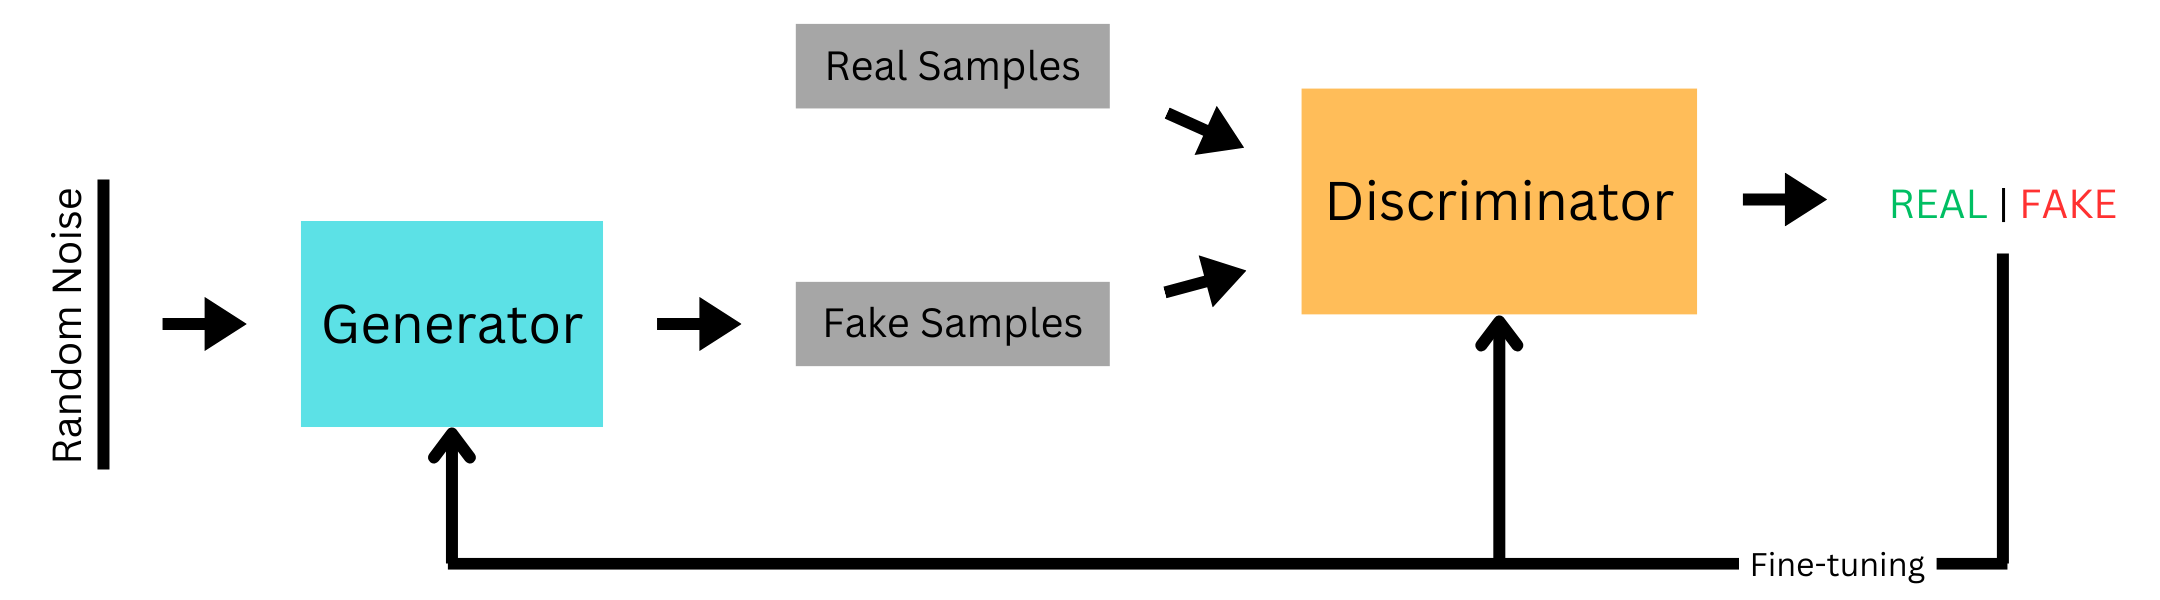
\includegraphics[width=1\columnwidth]{figures/Generator.png}
  \caption{Simplified functionality of a Generative Adversarial Network}\label{fig:figureGAN}
\end{figure}

Initially, the discriminator is trained on a dataset of unlabeled data, aiming to learn the characteristics and attributes of the desired output. Once it becomes proficient at identifying the genuine objects, it is presented with examples of non-objects and its ability to distinguish these examples is assessed. 
Subsequently, the generator utilizes random input vectors to generate counterfeit versions of the desired objects. 
The discriminator then assesses the authenticity of these outputs and shares the result. Based on this feedback, the generator or the discriminator adjust their behavior. This iterative process, facilitated by an iterator, involves creating samples, updating the models, and repeating the cycle. Gradually, the generator becomes highly skilled at producing realistic outputs that the discriminator can no longer distinguish from real ones. This process is referred to as a zero-sum game, where there is always a winner and a loser. The winner remains unchanged, while the loser updates its model based on the feedback received from the discriminator.

For Images, the Discriminator and the Generator are often implemented as Convolutional Neural Networks (CNNs), which excel at recognizing patterns in images and are commonly used for object identification.
GANs are not limited to images, they can also be applied to tasks such as video frame prediction, image enhancement to improve image quality, and encryption \citep{goodfellowGAN}.

GANs pose a substantial challenge in their training process as they are hard to train \citep{goodfellowGAN}. In addition, \citeauthor{brophyGAN} highlight three important problems commonly associated with GANs, among others. These issues, namely non-convergence, diminishing or vanishing gradients, and mode collapse, contribute to the inherent instability experienced during GAN training. Non-convergence refers to the failure of a GAN model to stabilize and reach a state of equilibrium. Instead, it continuously oscillates and fails to converge to a satisfactory solution. As a result, the model does not learn the underlying patterns of the data and can even diverge, leading to poor performance \citep{brophyGAN}. Diminishing or vanishing gradients occur when the gradients used to update the generator become extremely small or even vanish altogether. This phenomenon is often caused by an overly successful discriminator that becomes too adept at distinguishing real and fake samples. As a result, the generator struggles to learn from the feedback provided by the discriminator, impeding its ability to generate high-quality samples \citep{brophyGAN}. Mode collapse happens when the generator collapses, meaning it focuses on producing only a limited set of samples or outputs, typically lacking diversity and variety \citep{salimansNIPS}. In such cases, the generator fails to capture the full range of patterns and characteristics present in the training data, resulting in uniform and repetitive samples that do not adequately represent the true distribution \citep{brophyGAN}.
